\subsection{Speed}
\label{sec:eval_req_speed} 

\subsubsection{Configuration}

\begin{figure}[H]
    \includegraphics[width=14cm,frame]{figures/eval_req_speed.png}
  \caption{Evaluation Speed requirement}
\end{figure}

The 'Speed' requirement is used to calculate the probability of a target report having a speed error smaller than a defined threshold. The difference of the speed (test speed vs. speed based on reference positions) is calculated, and if its absolute value is smaller or equal than the defined threshold, the target report is counted for the calculated probability PCP (probability of check passed). The PCP must be greater or equal than the defined 'Probability' for the requirement to pass. \\

In another variation, if the 'Use Percent Threshold if Higher' checkbox is set, the check is changed for faster speeds. If the 'Threshold Percent' value times the calculated speed is larger or equal the defined threshold value, then the threshold value is changed to the value of the 'Threshold Percent' value times the calculated speed. This means that for higher speeds, an accuracy with the given percentage is required. \\

\begin{itemize}  
\item Probability [1]: Probability of correct speed
\item Probability Check Type: $\geq$
\item Speed Offset Value [m/s]: Maximum absolute speed difference between the test and the reference, in meters per second
\item Use Percent Threshold if Higher: Defines if the percent-based accuracy should be used for higher speeds
\item Threshold Percent [\%]: Percent threshold
\item Threshold Value Check Type: $\leq$, speed difference must be less or equal the given threshold
\item Failed Values are of Interest: Checked, the speed values of interest are the ones not passing the check
\end{itemize}
\ \\

\subsubsection{Result Values}

\paragraph{Sector}

\begin{center}
 \begin{table}[H]
  \begin{tabularx}{\textwidth}{ | l | X |  l | }
    \hline
    \textbf{Name} & \textbf{Description} & \textbf{Example} \\ \hline
    Sector Layer & Name of the sector layer & fir\_cut\_sim \\ \hline
    Reqirement Group & Name of the requirement group & Mandatory \\ \hline
    Requirement & Name of the requirement & Speed \\ \hline
    Num Results & Total number of results & 728 \\ \hline
    Num Usable Results & Number of usable results & 107 \\ \hline
    Num Unusable Results & Number of unusable results & 621 \\ \hline
    Use & To be used in results & true \\ \hline
    \#Pos [1] & Number of updates & 101685 \\ \hline
    \#NoRef [1] & Number of updates w/o reference speeds & 7359 \\ \hline
    \#PosInside [1] & Number of updates inside sector & 53997 \\ \hline
    \#PosOutside [1] & Number of updates outside sector & 40329 \\ \hline
    \#NoTstData [1] & Number of updates without tst speed data & 0 \\ \hline
    OMin [m/s] & Minimum of speed offset & 0.00 \\ \hline
    OMax [m/s] & Maximum of speed offset & 1114.58 \\ \hline
    OAvg [m/s] & Average of speed offset & 3.59 \\ \hline
    OSDev [m/s] & Standard Deviation of speed offset & 7.62 \\ \hline
    OVar [m$^2$/s$^2$] & Variance of speed offset & 58.01 \\ \hline
    \#CF [1] & Number of updates with failed comparison & 38 \\ \hline
    \#CP [1] & Number of updates with passed comparison  & 53959 \\ \hline
    PCP [\%] & Probability of passed comparison & 99.93 \\ \hline
    Condition &  & >= 90.00 \\ \hline
    Condition Fulfilled &  & Passed \\ \hline
\end{tabularx}
\end{table}
\end{center}

Also, a table is given for all single targets, sorted by PCP.

\paragraph{Single Target}

\begin{center}
 \begin{table}[H]
  \begin{tabularx}{\textwidth}{ | l | X |  l | }
    \hline
    \textbf{Name} & \textbf{Description} & \textbf{Example} \\ \hline
    Use & To be used in results & true \\ \hline
    \#Pos [1] & Number of updates & 1795 \\ \hline
    \#NoRef [1] & Number of updates w/o reference speeds & 131 \\ \hline
    \#PosInside [1] & Number of updates inside sector & 949 \\ \hline
    \#PosOutside [1] & Number of updates outside sector & 715 \\ \hline
    \#NoTstData [1] & Number of updates without tst speed data & 0 \\ \hline
    OMin [m/s] & Minimum of speed offset & 0.00 \\ \hline
    OMax [m/s] & Maximum of speed offset & 56.07 \\ \hline
    OAvg [m/s] & Average of speed offset & 5.23 \\ \hline
    OSDev [m/s] & Standard Deviation of speed offset & 5.60 \\ \hline
    OVar [m$^2$/s$^2$] & Variance of speed offset & 31.34 \\ \hline
    \#CF [1] & Number of updates with failed comparison & 2 \\ \hline
    \#CP [1] & Number of updates with  passed comparison & 947 \\ \hline
    PCP [\%] & Probability of passed comparison & 99.79 \\ \hline
    Condition &  & >= 90.00 \\ \hline
    Condition Fulfilled &  & Passed \\ \hline
\end{tabularx}
\end{table}
\end{center}

\subsection{Track Angle}
\label{sec:eval_req_track_angle} 

\subsubsection{Configuration}

\begin{figure}[H]
    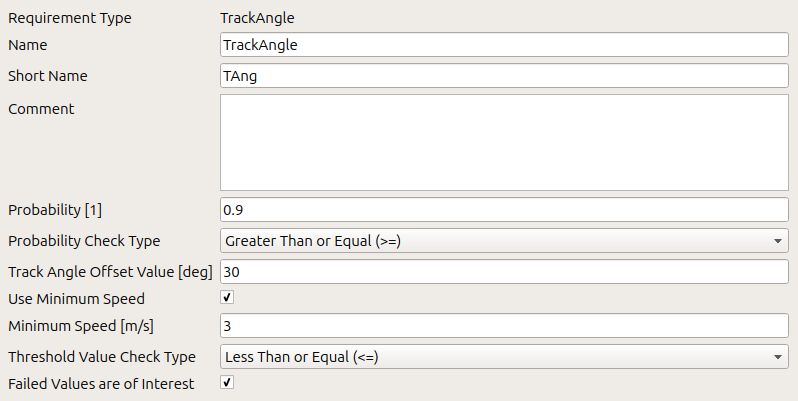
\includegraphics[width=14cm,frame]{figures/eval_req_track_angle.png}
  \caption{Evaluation Track Angle requirement}
\end{figure}

The 'Track Angle' requirement is used to calculate the probability of a target report having an track angle (direction of movement) error smaller than a defined threshold. Since this check only makes sense for moving targets, a minimum speed is defined, updates with less speed are ignored. The difference of the track angle (test vs. linear inpolated reference values) is calculated, and if its absolute value is smaller or equal than the defined threshold, the target report is counted for the calculated probability PCP (probability of check passed). The PCP must be greater or equal than the defined 'Probability' for the requirement to pass. \\

\begin{itemize}  
\item Probability [1]: Probability of correct track angle
\item Probability Check Type: $\geq$
\item Track Angle Offset Value [deg]: Maximum absolute difference between the test and the reference, in degrees
\item Use Minimum Speed: Defines if the minimum speed threshold shall be active
\item Minimum Speed [m/s]: Minimum speed for target reports to be checked
\item Threshold Value Check Type: $\leq$, differences must be less or equal the given threshold
\item Failed Values are of Interest: Checked, the values of interest are the ones not passing the check
\end{itemize}
\ \\

\subsubsection{Result Values}

\paragraph{Sector}

\begin{center}
 \begin{table}[H]
  \begin{tabularx}{\textwidth}{ | l | X |  l | }
    \hline
    \textbf{Name} & \textbf{Description} & \textbf{Example} \\ \hline
    Sector Layer & Name of the sector layer & units\_OPS\_2024 \\ \hline
    Reqirement Group & Name of the requirement group & Mandatory \\ \hline
    Requirement & Name of the requirement & TrackAngle \\ \hline
    Num Results & Total number of results & 1969 \\ \hline
    Num Usable Results & Number of usable results & 1491 \\ \hline
    Num Unusable Results & Number of unusable results & 478 \\ \hline
    Use & To be used in results & true \\ \hline
    \#Pos [1] & Number of updates & 581710 \\ \hline
    \#NoRef [1] & Number of updates w/o reference trackangles & 282 \\ \hline
    \#PosInside [1] & Number of updates inside sector & 581133 \\ \hline
    \#PosOutside [1] & Number of updates outside sector & 295 \\ \hline
    \#NoTstData [1] & Number of updates without tst trackangle data & 0 \\ \hline
    OMin [m/s] & Minimum of trackangle offset & -179.3 \\ \hline
    OMax [m/s] & Maximum of trackangle offset & 179.98 \\ \hline
    OAvg [m/s] & Average of trackangle offset & -0.01 \\ \hline
    OSDev [m/s] & Standard Deviation of trackangle offset & 5.25 \\ \hline
    OVar [$m^2$/$s^2$] & Variance of trackangle offset & 27.53 \\ \hline
    \#CF [1] & Number of updates with failed comparison & 2670 \\ \hline
    \#CP [1] & Number of updates with passed comparison & 577009 \\ \hline
    PCP [\%] & Probability of passed comparison & 99.54 \\ \hline
    Condition &  & >= 90.00 \\ \hline
    Condition Fulfilled &  & Passed \\ \hline
\end{tabularx}
\end{table}
\end{center}

Also, a table is given for all single targets, sorted by PCP.

\paragraph{Single Target}

\begin{center}
 \begin{table}[H]
  \begin{tabularx}{\textwidth}{ | l | X |  l | }
    \hline
    \textbf{Name} & \textbf{Description} & \textbf{Example} \\ \hline
    Use & To be used in results & true \\ \hline
    \#Pos [1] & Number of updates & 813 \\ \hline
    \#NoRef [1] & Number of updates w/o reference trackangles & 0 \\ \hline
    \#PosInside [1] & Number of updates inside sector & 813 \\ \hline
    \#PosOutside [1] & Number of updates outside sector & 0 \\ \hline
    \#NoTstData [1] & Number of updates without tst trackangle data & 0 \\ \hline
    OMin [m/s] & Minimum of trackangle offset & -7.82 \\ \hline
    OMax [m/s] & Maximum of trackangle offset & 7.92 \\ \hline
    OAvg [m/s] & Average of trackangle offset & 0.05 \\ \hline
    OSDev [m/s] & Standard Deviation of trackangle offset & 0.66 \\ \hline
    OVar [$m^2$/$s^2$] & Variance of trackangle offset & 0.44 \\ \hline
    \#CF [1] & Number of updates with failed comparison & 0 \\ \hline
    \#CP [1] & Number of updates with passed comparison & 813 \\ \hline
    PCP [\%] & Probability of passed comparison & 100.00 \\ \hline
    Condition &  & >= 90.00
    Condition Fulfilled;;Passed
\end{tabularx}
\end{table}
\end{center}


\subsection{Acceleration Correct}
\label{sec:eval_req_accel_correct} 

\subsubsection{Configuration}

\begin{figure}[H]
    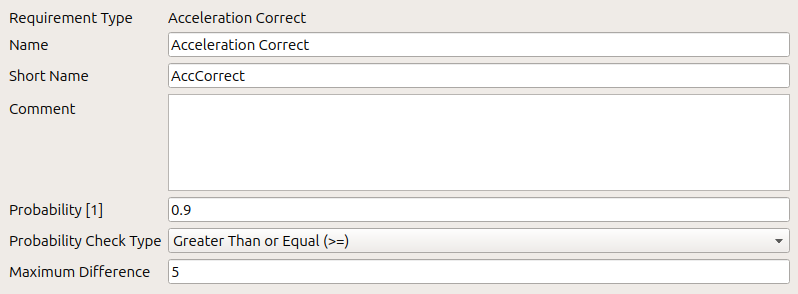
\includegraphics[width=14cm,frame]{figures/eval_req_acceleration.png}
  \caption{Evaluation Acceleration Correct Requirement}
\end{figure}

The ’Acceleration Correct’ requirement is used to calculate the probability of a target report having an acceleration error smaller than a defined threshold. 

\begin{itemize}  
\item Probability [1]: Probability of correct acceleration
\item Probability Check Type: $\geq$
\item Maximum Difference: Maximum difference in $m/s^2$
\end{itemize}
\ \\

\subsubsection{Calculation}

The offset of the acceleration (test vs. linear interpolated reference values) is used to calculate the offset. If the value of this offset fails the defined comparison threshold, the target report is counted for the calculated probability PCAcc (probability of correct acceleration). The PCAcc must be in turn pass the check for the requirement to pass. 

\subsubsection{Result Values}

\paragraph{Sector}

\begin{center}
 \begin{table}[H]
  \begin{tabularx}{\textwidth}{ | l | X |  l | }
    \hline
    \textbf{Name} & \textbf{Description} & \textbf{Example} \\ \hline
    Sector Layer & Name of the sector layer & units\_OPS\_2024 \\ \hline
    Reqirement Group & Name of the requirement group & Mandatory \\ \hline
    Requirement & Name of the requirement & Acceleration Correct \\ \hline
    Num Results & Total number of results & 1969 \\ \hline
    Num Usable Results & Number of usable results & 1492 \\ \hline
    Num Unusable Results & Number of unusable results & 477 \\ \hline
    Use & To be used in results & true \\ \hline
    \#Up [1] & Number of updates & 583549 \\ \hline
    \#NoRef [1] & Number of updates w/o reference position or Acceleration & 331 \\ \hline
    \#NoRefPos [1] & Number of updates w/o reference position & 282 \\ \hline
    \#NoRef [1] & Number of updates w/o reference Acceleration & 49 \\ \hline
    \#PosInside [1] & Number of updates inside sector & 582972 \\ \hline
    \#PosOutside [1] & Number of updates outside sector & 295 \\ \hline
    \#Unknown [1] & Number of updates unknown Acceleration & 0 \\ \hline
    \#Correct [1] & Number of updates with correct Acceleration & 578555 \\ \hline
    \#False [1] & Number of updates with incorrect Acceleration & 4368 \\ \hline
    PCAcc [\%] & Probability of Correct ACC & 99.25 \\ \hline
    Condition &  & >= 90.00 \\ \hline
    Condition Fulfilled &  & Passed \\ \hline
    \end{tabularx}
\end{table}
\end{center}

Also, a table is given for all single targets, sorted by PCAcc.

\paragraph{Single Target}

\begin{center}
 \begin{table}[H]
  \begin{tabularx}{\textwidth}{ | l | X |  l | }
    \hline
    \textbf{Name} & \textbf{Description} & \textbf{Example} \\ \hline
    Use & To be used in results & true \\ \hline
    \#Up [1] & Number of updates & 609 \\ \hline
    \#NoRef [1] & Number of updates w/o reference position or Acceleration & 0 \\ \hline
    \#NoRefPos [1] & Number of updates w/o reference position  & 0 \\ \hline
    \#NoRef [1] & Number of updates w/o reference Acceleration & 0 \\ \hline
    \#PosInside [1] & Number of updates inside sector & 609 \\ \hline
    \#PosOutside [1] & Number of updates outside sector & 0 \\ \hline
    \#Unknown [1] & Number of updates unknown Acceleration & 0 \\ \hline
    \#Correct [1] & Number of updates with correct Acceleration & 606 \\ \hline
    \#False [1] & Number of updates with incorrect Acceleration & 3 \\ \hline
    PCAcc [\%] & Probability of Correct ACC & 99.51 \\ \hline
    Condition &  & >= 90.00 \\ \hline
    Condition Fulfilled &  & Passed \\ \hline
\end{tabularx}
\end{table}
\end{center}
